%\documentclass[honours,12pt,twoside]{unswthesis}

\usepackage{afterpage}
\usepackage{amsfonts}
\usepackage{amsmath}
\usepackage{amssymb}
\usepackage{amsthm}
\usepackage[english]{babel}
\usepackage{graphicx}
\usepackage{natbib}
\usepackage[utf8]{inputenc}
\usepackage{latexsym}
\usepackage{url}
\usepackage{todonotes}
\usepackage{tikz}
\usepackage{pdfpages}
\usetikzlibrary{arrows}
\usepackage{float}
\usepackage[algoruled,boxed,lined]{algorithm2e}

\usepackage{booktabs}
\renewcommand{\arraystretch}{1.2}


%%%%%%%%%%%%%%%%%%%%%%%%%%%%%%%%%%%%%%%%%%%%%%%%%%%%%%%%%%%%%%%%%
%
%  The following are some simple LaTeX macros to give some
%  commonly used letters in funny fonts. You may need more or less of
%  these
%
\newcommand{\R}{\mathbb{R}}
\newcommand{\Q}{\mathbb{Q}}
\newcommand{\C}{\mathbb{C}}
\newcommand{\N}{\mathbb{N}}
\newcommand{\F}{\mathbb{F}}
\newcommand{\PP}{\mathbb{P}}
\newcommand{\T}{\mathbb{T}}
\newcommand{\Z}{\mathbb{Z}}
\newcommand{\B}{\mathfrak{B}}
\newcommand{\BB}{\mathcal{B}}
\newcommand{\M}{\mathfrak{M}}
\newcommand{\X}{\mathfrak{X}}
\newcommand{\Y}{\mathfrak{Y}}
\newcommand{\CC}{\mathcal{C}}
\newcommand{\E}{\mathbb{E}}
\newcommand{\cP}{\mathcal{P}}
\newcommand{\cS}{\mathcal{S}}
\newcommand{\A}{\mathcal{A}}
\newcommand{\ZZ}{\mathcal{Z}}

%%%%%%%%%%%%%%%%%%%%%%%%%%%%%%%%%%%%%%%%%%%%%%%%%%%%%%%%%%%%%%%%%%%%%
%
% The following are much more esoteric commands that I have left in
% so that this file still processes. Use or delete as you see fit
%
\newcommand{\bv}[1]{\mbox{BV($#1$)}}
\newcommand{\comb}[2]{\left(\!\!\!\begin{array}{c}#1\\#2\end{array}\!\!\!\right)
}
\newcommand{\Lat}{{\rm Lat}}
\newcommand{\var}{\mathop{\rm var}}
\newcommand{\Pt}{{\mathcal P}}
\def\tr(#1){{\rm trace}(#1)}
\def\Exp(#1){{\mathbb E}(#1)}
\def\Exps(#1){{\mathbb E}\sparen(#1)}
\newcommand{\floor}[1]{\left\lfloor #1 \right\rfloor}
\newcommand{\ceil}[1]{\left\lceil #1 \right\rceil}
\newcommand{\hatt}[1]{\widehat #1}
\newcommand{\modeq}[3]{#1 \equiv #2 \,(\text{mod}\, #3)}
\newcommand{\rmod}{\,\mathrm{mod}\,}
\newcommand{\p}{\hphantom{+}}
\newcommand{\vect}[1]{\mbox{\boldmath $ #1 $}}
\newcommand{\reff}[2]{\ref{#1}.\ref{#2}}
\newcommand{\psum}[2]{\sum_{#1}^{#2}\!\!\!'\,\,}
\newcommand{\bin}[2]{\left( \begin{array}{@{}c@{}}
				#1 \\ #2
			\end{array}\right)	}
%
%  Macros - some of these are in plain TeX (gasp!)
%
\newcommand{\be}{($\beta$)}
\newcommand{\eqp}{\mathrel{{=}_p}}
\newcommand{\ltp}{\mathrel{{\prec}_p}}
\newcommand{\lep}{\mathrel{{\preceq}_p}}
\def\brack#1{\left \{ #1 \right \}}
\def\bul{$\bullet$\ }
\def\cl{{\rm cl}}
\let\del=\partial
\def\enditem{\par\smallskip\noindent}
\def\implies{\Rightarrow}
\def\inpr#1,#2{\t \hbox{\langle #1 , #2 \rangle} \t}
\def\ip<#1,#2>{\langle #1,#2 \rangle}
\def\lp{\ell^p}
\def\maxb#1{\max \brack{#1}}
\def\minb#1{\min \brack{#1}}
\def\mod#1{\left \vert #1 \right \vert}
\def\norm#1{\left \Vert #1 \right \Vert}
\def\paren(#1){\left( #1 \right)}
\def\qed{\hfill \hbox{$\Box$} \smallskip}
\def\sbrack#1{\Bigl \{ #1 \Bigr \} }
\def\ssbrack#1{ \{ #1 \} }
\def\smod#1{\Bigl \vert #1 \Bigr \vert}
\def\smmod#1{\bigl \vert #1 \bigr \vert}
\def\ssmod#1{\vert #1 \vert}
\def\sspmod#1{\vert\, #1 \, \vert}
\def\snorm#1{\Bigl \Vert #1 \Bigr \Vert}
\def\ssnorm#1{\Vert #1 \Vert}
\def\sparen(#1){\Bigl ( #1 \Bigr )}

\newcommand\blankpage{%
    \null
    \thispagestyle{empty}%
    \addtocounter{page}{-1}%
    \newpage}
    
%%%%%%%%%%%%%%%%%%%%%%%%%%%%%%%%%%%%%%%%%%%%%%%%%%%%%%%%%%%%%%
%
% These environments allow you to get nice numbered headings
%  for your Theorems, Definitions etc.  
%
%  Environments
%
%%%%%%%%%%%%%%%%%%%%%%%%%%%%%%%
\newtheorem{theorem}{Theorem}[section]
\newtheorem{lemma}[theorem]{Lemma}
\newtheorem{proposition}[theorem]{Proposition}
\newtheorem{corollary}[theorem]{Corollary}
\newtheorem{conjecture}[theorem]{Conjecture}
%\theoremstyle{definition}
\newtheorem{definition}[theorem]{Definition}
\newtheorem{example}{Example}
\newtheorem{remark}[theorem]{Remark}
\newtheorem{question}[theorem]{Question}
\newtheorem{notation}[theorem]{Notation}
\numberwithin{equation}{section}

%\begin{document}

\chapter{Neural networks}\label{neuralNets-intro}

This chapter outlines the structure and workings of basic neural network models. Those who have a basic understanding of neural networks and wish to avoid the details surrounding model structure and minimisation algorithms can proceed to Chapter \ref{convnets} for an overview of convolutional neural networks and Chapter \ref{litrev} for existing lacune model attempts.

% - Basic neural networks theory + perceptron
% - Loss functions
% - Minimisation functions
% 
% - Convolutional neural networks overview
% - Convolution layer
% - ReLU
% - Pooling
% - Fully connected layers
% 
% - 3D CNNs overview

Neural networks have become increasingly popular with advances in computing power and the availability of large data sets \cite{Goodfellow-et-al-2016}. They have been proven successful with \textsc{mri} discrimination tasks \cite{DouQ.2016ADoC, Yokoyama2007} and image classification tasks \cite{AlexNet2012, GoogLeNet2015, HeKaiming2015DDiR}. In some instances, neural networks have exhibited a higher image recognition accuracy than humans \cite{HeKaiming2015DDiR}.

The construction of neural networks has to be conducted with care. The resulting models are difficult to interpret and prone to overfitting. We now discuss the underlying structure of neural networks, loss minimisation, and techniques to avoid overfitting the data.

\section{Basic structure}\label{nnets-structure}

The structure of neural networks can be compared to that of neurons in the brain. Each brain cell receives a signal, conducts a small amount of processing, and passes the resulting signal to the next cell. Decisions made by the brain are the result of many neurons processing information in sequence. Neural networks adopt a similar structure. Individual nodes receive variables, apply a transformation, and pass the result to the next node. For this reason, the nodes are referred to as \textit{neurons}.

The structure of a neural network neuron is shown in Figure \ref{nnet-neuronfig}. Let $\mathbf{x} = (x_1, x_2, \ldots, x_n)^\intercal$ be a vector of $n$ input variables. Let $\mathbf{w} = (w_1, \ldots, w_n)^\intercal$ be a vector of weights. Let $b$ be an additional \textit{bias} variable. This bias is not to be confused with statistical bias and is included to provide the neuron with a constant term. The output of a single neuron is given by
\[
	a = \sigma(\mathbf{w}\cdot\mathbf{x} + b),
\]
where $\sigma(\cdot)$ is an \textit{activation function} and $a$ is an \textit{activation value}.



% Neuron structure diagram
\begin{figure}
\centering
\tikzset{every picture/.style={line width=0.75pt}} %set default line width to 0.75pt        

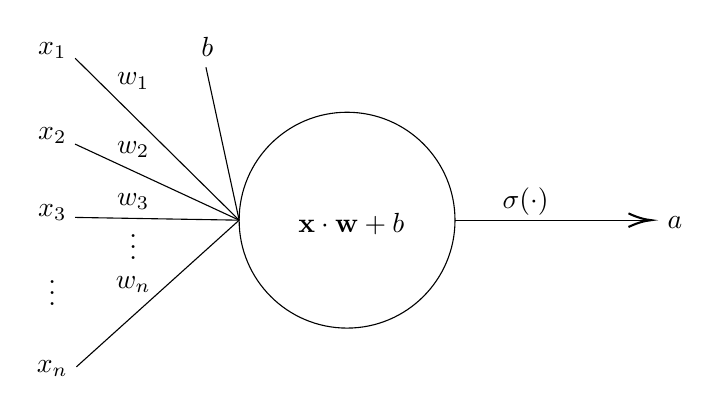
\begin{tikzpicture}[x=0.75pt,y=0.75pt,yscale=-1,xscale=1]
%uncomment if require: \path (0,300); %set diagram left start at 0, and has height of 300

%Shape: Circle [id:dp7806506925261892] 
\draw   (270,154) .. controls (270,125.28) and (293.28,102) .. (322,102) .. controls (350.72,102) and (374,125.28) .. (374,154) .. controls (374,182.72) and (350.72,206) .. (322,206) .. controls (293.28,206) and (270,182.72) .. (270,154) -- cycle ;
%Straight Lines [id:da48045113953293783] 
\draw    (191,76) -- (270,154) ;


%Straight Lines [id:da20730706323067383] 
\draw    (190.92,117.33) -- (270,154) ;


%Straight Lines [id:da19390293965519045] 
\draw    (191.59,224.67) -- (270,154) ;


%Straight Lines [id:da5499170807272789] 
\draw    (374,154) -- (466.51,154) ;
\draw [shift={(468.51,154)}, rotate = 180] [color={rgb, 255:red, 0; green, 0; blue, 0 }  ][line width=0.75]    (10.93,-3.29) .. controls (6.95,-1.4) and (3.31,-0.3) .. (0,0) .. controls (3.31,0.3) and (6.95,1.4) .. (10.93,3.29)   ;

%Straight Lines [id:da7426731370805287] 
\draw    (270,154) -- (190.92,152.67) ;


%Straight Lines [id:da35133187079282135] 
\draw    (254,80.33) -- (270,154) ;



% Text Node
\draw (324,156) node   {$\mathbf{x} \cdot \mathbf{w} +b$};
% Text Node
\draw (180,72.33) node   {$x_{1}$};
% Text Node
\draw (180,113.33) node   {$x_{2}$};
% Text Node
\draw (180,185) node   {$\vdots $};
% Text Node
\draw (180,225.33) node   {$x_{n}$};
% Text Node
\draw (180,150.33) node   {$x_{3}$};
% Text Node
\draw (219,87) node   {$w_{1}$};
% Text Node
\draw (219,120) node   {$w_{2}$};
% Text Node
\draw (219,145) node   {$w_{3}$};
% Text Node
\draw (219,185) node   {$w_{n}$};
% Text Node
\draw (219,163) node   {$\vdots $};
% Text Node
\draw (254.67,70.33) node   {$b$};
% Text Node
\draw (408,145) node   {$\sigma ( \cdot )$};
% Text Node
\draw (480,155) node   {$a$};


\end{tikzpicture}
\caption{Neuron structure.}
\label{nnet-neuronfig}
\end{figure}






%% Diagram of single neuron
%\begin{figure}[ht]
%	\centering
%	\includegraphics[scale=0.5]{Images/3_neuron.png}
%	\caption{Neuron structure.}
%	\label{nnet-neuronfig}
%\end{figure}

A large number of these neurons can be arranged to form a neural network. The generated outputs of these neurons can be fed as inputs into later neurons. Basic neural networks arrange a number of these neurons into layers, as shown in Figure \ref{nnet-structurefig}. The first layer is an input layer, where data is fed into the model. Each neuron in this first layer represents a variable. The last layer is an output layer which generates the final result. The central layers, which conduct most of the processing, are known as \textit{hidden layers}.

% Diagram of basic neural network structure. Input, 1 hidden layer and series of output layers
%\begin{figure}[ht]
%	\centering
%	\includegraphics[width=\textwidth]{Images/3_nnet_structure.jpg}
%	\caption{Basic neural network structure.}
%	\small Image taken from \url{`https://www.digitaltrends.com/cool-tech/what-is-an-artificial-neural-network/'}
%	\label{nnet-structurefig}
%\end{figure}
\begin{figure}
\centering
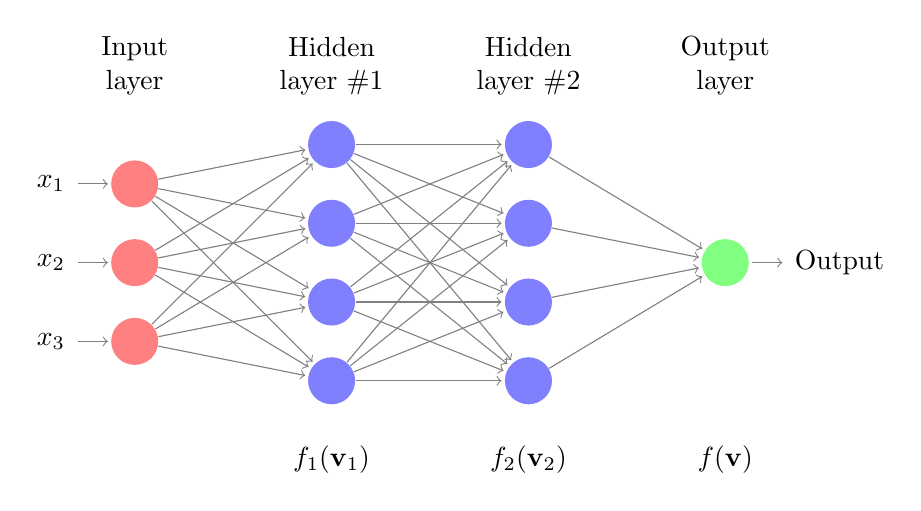
\begin{tikzpicture}[shorten >=1pt,->,draw=black!50, node distance=\layersep]
    \tikzstyle{every pin edge}=[<-,shorten <=1pt]
    \tikzstyle{neuron}=[circle,fill=black!25,minimum size=17pt,inner sep=0pt]
    \tikzstyle{input neuron}=[neuron, fill=red!50];
    \tikzstyle{output neuron}=[neuron, fill=green!50];
    \tikzstyle{hidden neuron}=[neuron, fill=blue!50];
    \tikzstyle{annot} = [text width=4em, text centered]
	\def\layersep{2.5cm}
	
    % Draw the input layer nodes
    \foreach \name / \y in {1,...,3}
    % This is the same as writing \foreach \name / \y in {1/1,2/2,3/3,4/4}
        \node[input neuron, pin=left:$x_\y$] (I-\name) at (0,-\y) {};

    % Draw the hidden layer1 nodes
    \foreach \name / \y in {1,...,4}
        \path[yshift=0.5cm]
            node[hidden neuron] (Ha-\name) at (\layersep,-\y cm) {};
            
    % Draw the hidden layer2 nodes
    \foreach \name / \y in {1,...,4}
        \path[yshift=0.5cm]
            node[hidden neuron] (Hb-\name) at (2*\layersep,-\y cm) {};

    % Draw the output layer node
    \node[output neuron,pin={[pin edge={->}]right:Output}] (O) at (3*\layersep, -2) {};

    % Connect every node in the input layer with every node in the
    % hidden layer.
    \foreach \source in {1,...,3}
        \foreach \dest in {1,...,4}
            \path (I-\source) edge (Ha-\dest);
            
    % Connect every node in the hidden layer 1 with every node in
    % hidden layer 2.
    \foreach \source in {1,...,4}
        \foreach \dest in {1,...,4}
            \path (Ha-\source) edge (Hb-\dest);

    % Connect every node in the hidden layer with the output layer
    \foreach \source in {1,...,4}
        \path (Hb-\source) edge (O);

    % Annotate the layers
    \node[annot,above of=Ha-1, node distance=1cm] (hla) {Hidden layer \#1};
    \node[annot,above of=Hb-1, node distance=1cm] (hlb) {Hidden layer \#2};
    \node[annot,left of=hla] {Input layer};
    \node[annot,right of=hlb] {Output layer};
    
    \node[annot,below of=Ha-4, node distance=1cm] (fa) {$f_1(\mathbf{v}_1)$};
    \node[annot,below of=Hb-4, node distance=1cm] (fb) {$f_2(\mathbf{v}_2)$};
    \node[annot,right of=fb, node distance=\layersep] (fo) {$f(\mathbf{v})$};

\end{tikzpicture}
\caption{Basic neural network structure. Each hidden neuron (blue) and the output neuron (green) has the structure shown in Figure \ref{nnet-neuronfig}. For simplicity, the weights and biases have been hidden.}
\label{nnet-structurefig}
\end{figure}

Let the weights and biases of layer $\ell$ be $\mathbf{v}_\ell$ and let the output of hidden layer $\ell$ be $f_\ell(\mathbf{v}_\ell)$. Then the output of the whole network is
\[
	f(\mathbf{v}) = f_L(\mathbf{v}_L) \circ f_{L-1}(\mathbf{v}_{L-1}) \circ \ldots \circ f_1(\mathbf{v}_1).
\]

All the weights $W$ and biases $B$ of the network are chosen such that they minimise some \textit{cost function} $C(W,B)$ with respect to $(W,B)$. However, since the number of variables can be very large, it is not always feasible to analytically minimise $C(W,B)$.

We can instead approximate this minimisation via the Gradient-Descent algorithm (see Section \ref{nnets-graddesc}). This algorithm is run until the cost function falls within some tolerance $\tau$, or reaches the maximum number of iterations $n_T$.

\section{Notation}\label{nnets-not}

\todo[inline]{Restructure notation like a glossary. Two columns, notation on left and definition on right.}

Let $\mathbf{w}^\ell_j$ to be the vector of weights used to compute the $j$-th neuron of the $\ell$-th layer, where $w_{ji}^\ell$ is the weight attributed to the $i$-th neuron of the $(\ell-1)$-th layer.

Let $b_j^\ell$ be the bias of the $j$-th neuron in the $\ell$-th layer.

Let $\mathbf{a}^\ell$ be the vector of activation values (outputs) for the $\ell$-th layer, where $a_j^\ell$ is the activation value of the $j$-th neuron of that layer. Set $z_j^\ell := \mathbf{w}_j^\ell\cdot \mathbf{a}^{\ell-1} + b_j^\ell= \sum_k w_{jk}^\ell a_k^{\ell-1} + b_j^\ell$ to be the values calculated before activation, and $\mathbf{z}^\ell$ to be the vector of $z_j^\ell$ for the $\ell$-th layer. Set $Z$ to be the set of all $z_j^\ell$ in the whole network. Let $L$ be the number of layers in the network so that $\mathbf{a}^L$ is the vector of activation values of the final output layer. Let $X = \{\mathbf{x}_1, \mathbf{x}_2, \ldots, \mathbf{x}_n\}$ be the set of $n$ training inputs. Let the responses be $Y = \{\mathbf{y}_1, \mathbf{y}_2, \ldots, \mathbf{y}_n\}$, with $y_{ij}$ the $j$-th variable of $\mathbf{y}_i$. Let $W$ and $B$ be the sets of all weights and biases as before. Let $\eta$ be the learning rate of the network. 

\section{Activation functions}\label{nnets-act}

Activation functions, denoted by $\sigma(\cdot)$, are applied just before neuron output. Without these functions, the network can be reduced to a linear combination of inputs. Activation functions serve to introduce nonlinearity into the model.

The simplest neuron type is called the \textit{perceptron}. In this neuron, the activation function is the step function,
\[
	x_i \in \{0,1\} \text{ and } \sigma(z) = \begin{cases}
		1 & z > 0 \\
		0 & z \le 0
	\end{cases}.
\]

To allow for continuous outputs, other common activation functions include the sigmoid function
\[
	\sigma(z) = \dfrac{1}{1+e^{-z}},
\]
and hyperbolic tan function,
\[
	\sigma(z) = \tanh(z),
\]
which are smooth approximations to a step activation function.

The Rectified Linear Unit (ReLU) activation is given by,
\[
	\sigma(z) = \max(0, z),
\]
which allows for some neurons to output 0 and be essentially deactivated.

A common activation function for the final layer is the softmax function,
\[
	\sigma(z_j) = \dfrac{e^{z_j}}{\sum_ke^{z_k}},
\]
as the output takes the form of a probability distribution.


\section{Cost functions}\label{nnets-cost}

Weights and biases are chosen such that they approximately minimise some cost function. To use the gradient descent algorithm (see Section \ref{nnets-graddesc}) to minimise cost, Nielson \cite{Nielson2015} describes two requirements. The first requirement is that the cost $C_X(\cdot)$ accrued from all samples $X$ equals the mean of costs accrued from $n$ distinct subsamples of $X$, denoted by $X_i$,
\[
	C_X(W, B) = \dfrac{1}{n}\sum_{i=1}^n C_{X_i}(W,B).
\]

The second requirement is that the cost is independent of $\mathbf{a}^\ell$ for all $\ell < L$. There are a number of cost functions in frequent use, and the choice of cost function is dependent on the context of the problem. A common cost function for regression is the quadratic cost, or Mean Squared Error (\textsc{mse}) cost. Denote $\|\cdot\|$ to be the Euclidean norm. The \textsc{mse} cost function is given by
\[
	C(W,B) = \dfrac{1}{2n}\sum_{i=1}^n||\mathbf{a}^L(\mathbf{x}_i,W,B) - \mathbf{y}_i ||^2.
\]
This form is convenient for backpropagation (see Section \ref{nnets-backprop}) as it has an efficiently computable gradient,
\[
	\nabla_aC = \dfrac{1}{n}\sum_{i=1}^n||\mathbf{a}^L(\mathbf{x}_i,W,B) - \mathbf{y}_i ||.
\]
In using quadratic cost, if the amount of error is large, the learning rate is low.

The most common cost function for classification tasks is cross entropy, given by
\[
	C(W,B) = -\dfrac{1}{n}\sum_{i=1}^n\sum_j\big[y_{ij}\log\big(a_j^L(\mathbf{x}_i,W,B)\big) + (1 - y_{ij})\log\big( (1 - a_j^L(\mathbf{x}_i,W,B))\big)\big],
\]
with gradient
\[
	\nabla_aC = \dfrac{1}{n}\sum_{i=1}^n\sum_j\dfrac{a_j^L(\mathbf{x}_i,W,B) - y_{ij}}{a_j^L(\mathbf{x}_i,W,B)(1-a_j^L(\mathbf{x}_i,W,B))}.
\]
Unlike the quadratic cost, when the error is high, the learning rate is also high.

%Cost functions can include: the quadratic (simple), cross-entropy, regularisation (L1, L2, dropout, artificial expansion of training data).
%In using cross-entropy, the learning rate of the weight is controlled by the amount of error. This is unlike the quadratic cost function, which has a very slow learning rate when there is high error.
%Changing these can improve a model.
%Other improvements made by making better initialisations of weights, and better heuristics to choose hyper-parameters.

\section{Gradient descent}\label{nnets-graddesc}

Weights and biases are chosen to minimise the cost function. Analytically minimising the cost function is possible, however the large number of variables makes this process slow, having time complexity $O(n^3)$ \cite{Marquardt1963}. To improve computation speed, the weights are instead estimated using the Gradient Descent algorithm.

Gradient Descent works by considering the gradient of the cost given the current weights and biases \cite{Nielson2015}. The algorithm shifts the weights and biases by a small amount such that the cost will decrease. The amount that the values shift by is referred to as the learning rate, denoted $\eta$ as before.

Let $N$ be a positive integer. For all weights and biases denoted $\mathbf{v}$, the change in cost $C(\mathbf{v})$ is given by the \textit{Total Differential Approximation},
\begin{align*}
	\Delta C(\mathbf{v}) & \approx \dfrac{\partial C}{\partial v_1}\Delta v_1 + \dfrac{\partial C}{\partial v_2}\Delta v_2 + \cdots + \dfrac{\partial C}{\partial v_N}\Delta v_N\\
	& = \nabla C(\mathbf{v})\cdot \Delta \mathbf{v},
\end{align*}
where $\nabla C(\mathbf{v}) = \Big(\dfrac{\partial C}{\partial v_1}, \dfrac{\partial C}{\partial v_2},\ldots, \dfrac{\partial C}{\partial v_N}\Big)$.

We define $\mathbf{v}'$ to be the updated value of $\mathbf{v}$. We update $\mathbf{v}'$ inductively such that the cost decreases by an amount proportional to $\eta$.

The next values of $\mathbf{v}$ are chosen such that the cost will decrease by an amount controlled by $\eta$, such that
\[
	\Delta\mathbf{v} = -\eta \nabla C(\mathbf{v}), \quad \text{ where }\eta > 0.
\]
By substitution, we can write
\[
	\Delta C(\mathbf{v}) \approx -\eta \|\nabla C(\mathbf{v})\|^2 \le 0,
\]
where $\|\cdot\|$ is the Euclidean norm.

Thus if $\mathbf{v}' := \mathbf{v} - \eta \nabla C(\mathbf{v})$, the cost will decrease.

In training a neural network, the size of the shift can be set to $\|\Delta\mathbf{v}\| = \varepsilon$, for some $\varepsilon > 0$. It can be shown that the $\Delta\mathbf{v}$ which gives the greatest decrease in $C(\mathbf{v})$ is a function of $\varepsilon$ and $\nabla C$ \cite{Nielson2015}.

\begin{proposition}\label{nnets-graddescminproof}
	Let $\varepsilon > 0$ and suppose the size of the shift is constrained such that $\|\Delta\mathbf{v}\| = \varepsilon$. Then $\nabla C \cdot \Delta\mathbf{v}$ is minimised by $\Delta\mathbf{v} = -\eta\nabla C$, where $\eta = \dfrac{\varepsilon}{\|\nabla C\|}$.
\end{proposition}

\begin{proof}
	Using the Cauchy-Schwarz Inequality,
	\[
			|\nabla C\cdot\Delta\mathbf{v}| \le \|\nabla C\|\cdot\|\Delta\mathbf{v}\|.
	\]
	Then the minimum is given by, \begin{align*}
		\min(\nabla C\cdot\Delta\mathbf{v}) & = -\|\nabla C\|\times\|\Delta\mathbf{v}\| \\
		& = -\varepsilon\|\nabla C\| \\
		& = -\dfrac{\varepsilon\|\nabla C\|^2}{\|\nabla C\|} \\
		& = -\dfrac{\varepsilon\nabla C\cdot\nabla C}{\|\nabla C\|}.
	\end{align*}
	Then by equating the coefficients of $\nabla C$,
	\begin{align*}
		\operatorname*{arg\,min}_{\Delta\mathbf{v}}(\nabla C\cdot\Delta\mathbf{v}) & = -\dfrac{\varepsilon\nabla C}{\|\nabla C\|} \\
		& = -\eta\nabla C,\quad\text{ where }\eta = \dfrac{\varepsilon}{\|\nabla C\|}.
	\end{align*}
\end{proof}

As gradient descent moves the coefficients in the direction of the steepest negative gradient, it assumes that the starting values are close enough to the global minimum to converge. If this assumption is not satistifed, the algorithm will instead converge to the local minimum. However, it is not possible to confirm whether the weights are converging to the global minimum or not.

%To address this, it is commonplace to initialise the weights randomly.
%
%A common distribution for initialising weights is the truncated normal distribution, which has the shape of the normal distribution $\mathcal{N}(\mu, \sigma^2)$, but is bounded such that $X\in(a,b),-\infty\le a < b\le \infty$.

As the updated weights and biases rely on the gradient, it should be noted that these gradients are then required to be significantly different from zero. When this is not the case, we have what is called the Vanishing Gradient Problem, which is discussed further in section \ref{nnet-vanishinggradprob}.

\subsection*{Stochastic gradient descent}\label{nnets-stochgraddesc}

As the neural network has a very large number of weights, gradient descent is a highly computationally intensive algorithm. To improve training time, Stochastic Gradient Descent is a popular alternative, shown to have a time complexity of $O(n)$ \cite{Robbins1951}. This algorithm improves learning speed by randomly selecting a small number of training inputs to learn from, referred to as a \textit{batch}. After training has been completed for that batch, another batch of training inputs is randomly selected, and the process repeats. When all training batches have been used, it is said that an \textit{epoch} of training has been completed.

In this manner, a relatively small number of samples is used for each weight adjustment. This drastically increases training speed, while still utilising all the information provided by the whole set of samples by the end of training time.

\subsection*{Adam optimiser}\label{nnets-adam}

The stochastic gradient algorithm maintains one learning rate for all of the weights in the network. The Adam Optimiser alters this algorithm by storing different learning rates for each of the parameters. 

%
%We attempt to choose weights and biases that will minimise the cost function. As we cannot use calculus, we must estimate - by gradient descent. Move all the estimates a little, in the direction of decrease. The amount of movement is dependent on a learning rate parameter.
%
%This takes a long time with all inputs. Stochastic gradient descent instead randomly choosing $m$ training inputs, known as a mini-batch. It trains with the mini-batch, then rechooses $m$ different, unused inputs, re-trains, etc. When there are no more inputs to choose from, the algorithm has completed an 'epoch' of training.
%
%Backpropagation: gradient of the cost function. 

\subsection*{Learning rate}\label{nnets-learningrate}

The learning rate, given by $\eta$, controls the adjustment of weights during training. As in Section \ref{nnets-graddesc}, the change in gradients, $\Delta\mathbf{v} = -\eta\nabla C$, moves the weights in the direction of the steepest negative gradient. $\eta$ then controls the magnitude of the movement.

The size of $\eta$ controls how quickly the model learns. If $\eta$ is too small, training will take a long time. If $\eta$ is too large, the model may move the weights too far, and the values of $\mathbf{v}$ will move past the local minimum.

To aid in efficient training, learning rates can be adjusted throughout. At the start of training, it can be beneficial to have a higher learning rate. This allows the weights to move closer to the local minimum much faster. At later epochs, a smaller learning rate will allow for fine tuning of the weights, ensuring precision. A common technique is to lower the learning rate only when validation accuracy drops.

\section{Backpropagation}\label{nnets-backprop}

During gradient descent, it is necessary to calculate the gradient of the cost function. This is done through backpropagation. This algorithm determines $\dfrac{\partial C}{\partial z}$, then relates those values to the rates of interest, $\dfrac{\partial C}{\partial W}$ and $\dfrac{\partial C}{\partial B}$. To describe the algorithm, we first need to derive some results.

% http://neuralnetworksanddeeplearning.com/chap2.html

\begin{proposition}
	The error of the jth neuron of the final output layer is
	\[
		\delta_j^L = \dfrac{\partial C}{\partial a_j^L}\sigma'(z_j^L).
	\]
	This can be expressed in the matrix form,
	\[
		\delta^L = \Sigma'(\mathbf{z}^L)\nabla_aC,
	\]
where $\Sigma'(\cdot)$ is a matrix where the $j$-th diagonal entry is $\sigma'(z_j^L)$ and all non-diagonal entries are 0.
\end{proposition}

\begin{proof}
	\begin{align*}
		\delta_j^L & = \dfrac{\partial C}{\partial z_j^L} \\
		& = \sum_k\dfrac{\partial C}{\partial a_k^L}\dfrac{\partial a_k^L}{\partial z_j^L} \\
		& = \dfrac{\partial C}{\partial a_j^L}\dfrac{\partial a_j^L}{\partial z_j^L}\text{, as }z_j^L\text{ is only a function of }a_k^L\text{ for }k = j \\
		& = \dfrac{\partial C}{\partial a_j^L}\sigma'(z_j^L).
	\end{align*}
\end{proof}

\begin{proposition}
	The error $\delta^\ell_j$ can be written in terms of the errors in the next layer, 
	\begin{align*}
		\delta_j^\ell & = \sum_k\delta_k^{\ell+1}w_{kj}^{\ell+1}\sigma'(z_j^\ell).
	\end{align*}
\end{proposition}

\begin{proof}
	Using the chain rule,
	\begin{align*}
		\delta_j^\ell & = \dfrac{\partial C}{\partial z_j^\ell} \\
		& = \sum_k\dfrac{\partial C}{\partial z_k^{\ell+1}}\dfrac{\partial z_k^{\ell+1}}{\partial z_j^\ell} \\
		& = \sum_k\delta_k^{\ell+1}\dfrac{\partial z_k^{\ell+1}}{\partial z_j^\ell}.
	\end{align*}
	Then as $\dfrac{\partial z_k^{\ell+1}}{\partial z_j^\ell} = \dfrac{\partial}{\partial z_j^\ell}(\mathbf{w}_k^{\ell+1}\cdot\sigma(\mathbf{z}^\ell) + b_k^{\ell+1}) = w_{kj}^{\ell+1}\sigma'(z_j^\ell)$,
	\begin{align*}
		\delta_j^\ell & = \sum_k\delta_k^{\ell+1}w_{kj}^{\ell+1}\sigma'(z_j^\ell).
	\end{align*}
\end{proof}


Together, the errors of layer $l$ can be written
\begin{align*}
	\delta^\ell & = \Sigma'(\mathbf{z}^\ell)(w^{\ell+1})^\intercal\delta^{\ell+1} \\
	& = \Sigma'(\mathbf{z}^\ell)(w^{\ell+1})^\intercal\ldots\Sigma'(\mathbf{z}^{L-1})(w^L)^\intercal\Sigma'(\mathbf{z}^L)\nabla_aC.
\end{align*}

\begin{proposition}
	The error $\delta_j^\ell$ is equivalent to the rate of change in cost with respect to the bias, so that
	\[
		\delta_j^\ell = \dfrac{\partial C}{\partial b_j^\ell}.
	\]
\end{proposition}
\begin{proof}
	By definition,
	\[
		\delta_j^\ell = \dfrac{\partial C}{\partial z_j^\ell}.
	\]
	Then by the chain rule,
	\[
		\delta_j^\ell = \sum_k\dfrac{\partial C}{\partial b_k^\ell}\dfrac{\partial b_k^\ell}{\partial z_j^\ell}.
	\]
	Then as $z_j^\ell$ is only a function of $b_k^\ell$ for $j = k$,
	\begin{align*}
		\delta_j^\ell & = \dfrac{\partial C}{\partial b_j^\ell}\dfrac{\partial b_j^\ell}{\partial z_j^\ell} \\
		& = \dfrac{\partial C}{\partial b_j^\ell}.
	\end{align*}
\end{proof}

\begin{proposition}
	The rate of change in cost with respect to any single weight value is given by
	\[
		\dfrac{\partial C}{\partial w_{jk}^\ell} = a_k^{\ell-1}\delta_j^\ell.
	\]
\end{proposition}
\begin{proof}
	By definition,
	\begin{align*}
		z_k^\ell & = \mathbf{w}_k^\ell\cdot\mathbf{a}^{\ell-1} + b_k^\ell \\
		& = \sum_jw_{kj}^\ell a_j^{\ell-1} + b_k^\ell.
	\end{align*}
	Then differentiating with respect to some weight $w_{km}^\ell$,
	\[
		\dfrac{\partial z_k^\ell}{\partial w_{km}^\ell} = a_m^{\ell-1}.
	\]
	Then using the Chain Rule,
	\begin{align*}	
		\dfrac{\partial C}{\partial w_{jk}^\ell} & = \dfrac{\partial C}{\partial z_j^\ell}\dfrac{\partial z_j^\ell}{\partial w_{jk}^\ell} \\
		& = \delta_j^\ell a_k^{\ell-1}.
	\end{align*}
\end{proof}


Using these equations, the backpropagation algorithm runs as follows:
\begin{enumerate}
	\item \textbf{Inputs}. Enter observations $x$ to retrieve $\mathbf{a}^1$.
	\item \textbf{Feedforward}. Compute the $\mathbf{z}^\ell = \mathbf{w}^\ell\mathbf{a}^{\ell-1} + \mathbf{b}^\ell$ for each $l = 2, 3,\ldots,L$.
	\item \textbf{Output error}. Compute $\delta^L = \Sigma'(\mathbf{z}^L)\nabla_aC$.
	\item \textbf{Backpropagation}. For $\ell = L-1, \ldots, 2$, compute $\delta^\ell =  \Sigma'(\mathbf{z}^\ell)(w^{\ell+1})^\intercal\delta^{\ell+1}$.
	\item \textbf{Gradients}. Compute $\dfrac{\partial C}{\partial b_j^\ell} = \delta_j^\ell$ and $\dfrac{\partial C}{\partial w_{jk}^\ell} = a_k^{\ell-1}\delta_j^\ell$.
\end{enumerate}


\subsection*{Vanishing gradient problem}\label{nnet-vanishinggradprob}
We note that the error, $\delta^\ell$, is dependent on the gradient of the activation function. If the gradient of the activation is close to 0, then both the error detected and learning rate also become close to 0.

\noindent For the sigmoid activation function,
\[
	\sigma '(z) = e^{-z}(1+e^{-z})^{-2}.
\]
For the tanh activation function,
\[
	\sigma '(z) = 1-\tanh^2(z).
\]
For both the sigmoid and tanh activations, the limit as $z\rightarrow\pm\infty$ yields 
\[
	\lim_{z\rightarrow\pm\infty}\sigma '(z)= 0.
\]
For the sigmoid and tanh activation functions, very large or very small $z_j^\ell$ will have near zero gradients. In this scenario, the training of weights and biases shift by smaller and smaller increments, so that further training does not improve the model over time.

A common alternative to these is the ReLU activation function. This activation has gradient
\[
	\sigma '(z) = \begin{cases}
		1 & z > 0 \\
		0 & z < 0
	\end{cases}.
\]
% Paper: https://www.utc.fr/~bordesan/dokuwiki/_media/en/glorot10nipsworkshop.pdf
Neurons that are active will have a constant gradient of 1. If the value of $z$ becomes negative, the neurons will stop training. If this occurs in the whole network, the ReLU activation can be replaced with the \textit{leaky ReLU},
\[
	\sigma(z) = \max(x, ax), \quad a \le 1.
\]
This activation has gradient function
\[
	\sigma '(z) = \begin{cases}
		1 & z > 0 \\
		a & z < 0
	\end{cases},
\]
which avoids the zero gradient for negative $z$.

\section{Weight initialisation}

The initialisation of weights and biases affects the rate and quality of training. Intuitively, if the weights are initialised close to the final output values, it will be faster to train. Conversely, weights that are initialised poorly will take a long time to train to the same accuracy, or may not converge to an appropriate solution.

If the weights of two nodes are similar, using the same activation function will result in similar outputs. Initialising weights and biases the same way introduces a lot of redundant calculations. 

It is commonplace for weights and biases to be initialised randomly. A common distribution for weight initialisation is the truncated normal distribution. Let $X\sim\mathcal{N}(\mu,\sigma^2)$ and $-\infty \le a < b \le \infty$. The truncated normal $X$ has probability density function
\[
	f_X(x;\mu, \sigma^2,a,b) = \dfrac{\phi\big(\frac{x-\mu}{\sigma}\big)}{\sigma\bigg(\Phi\big(\frac{b-\mu}{\sigma}\big) - \Phi\big(\frac{a-\mu}{\sigma}\big)\bigg)}\quad \text{ if } x \in (a,b) \text{ and 0 otherwise,}
\]
where $\phi$ and $\Phi$ are the standard normal probability density function and cumulative density functions respectively.

Another common weight initialisation method is the He Method \cite{HeKaiming2015DDiR}. This method recognises the use of the ReLU activation function. Initial values are dependent on the size of the previous layer.

He Method initialisation is given by
\[
	w = Z\times\sqrt{\dfrac{2}{d_{\ell-1}}},\quad Z\sim\mathcal{N}(0,1),
\]
where $d_{\ell-1}$ is the number of nodes in the $(\ell-1)$th layer.

%Initial weights and biases chosen using independent Gaussian random variables, with mean 0, sd 1. But this is quite a broad distribution. Can become relatively likely for neurons to become saturated (corrections are minuscule). Instead, try a standard deviation of $1/\sqrt(n)$.

%Choosing hyper-parameters:
%It can be difficult to determine what to change with so many parameters in play at once. This is particularly the case with large amounts of data or complex models. Change the learning rate? Number of hidden neurons? Number of layers? 
%General strategy is to start simple. First just try to get ANY non-trivial result. E.g. for MNIST, just isolate 0/1 images. Start without hidden layers, just to test it out. Once there are non-trivial results, start building these more complex structures.

\section{Regularisation}\label{nnet-reg}

Neural networks contain a very large number of parameters to be estimated. Parameters generally outnumber observations, so observations have to be reused when calculating parameter estimates. Hence neural networks have a tendency to overfit the data. One common method to mitigate this is to apply penalties to the calculation of cost. This is called \textit{regularisation}.

\subsection*{L2-regularisation}\label{nnet-l2reg}

% Regularisation & Dropout

\textit{L2-regularisation}, also known as Ridge Regression, adds an extra penalty term to the cost function. The cost function becomes
\[
	C(W,B) + \dfrac{\lambda}{2n}\sum_{w\in W}w^2.
\]
The penalty term is scaled by $\lambda$, known as the regularisation parameter. 

Another common regularisation is L1, or Lasso Regression, which takes the sum of the absolute weights,
\[
	C(W,B) + \dfrac{\lambda}{n}\sum_{w\in W}|w|.
\]

\subsection*{Dropout}\label{nnet-dropout}

Through the training process, it is possible for individual neurons to become sensitive to patterns present in specific observations. When a dropout layer is added, each neuron connected to the layer has a preset probability $p$ of being deactivated, regardless of their input. This ensures that relevant features of the data are spread through several neurons, and that the impact of an individual neuron does not strongly affect the final result.

\subsection*{Batch normalisation}

After a large amount of training time, particular activation values can become very large or very small. Normalising the activations within each batch stops the values from becoming too extreme, allowing for some additional features to train. Similarly to dropout, batch normalisation also avoids overfitting by adding some noise to the weights and ensuring that critical features are spread across nodes.

\subsection*{Data expansion}

Neural networks require a very large sample size to avoid overfitting as there are a large number of variables. If the number of samples is not large enough, the data can be augmented and added to the existing dataset, introducing more varied samples.

Common augmentations for image data include flipping horizontally and vertically, rotation and cropping. It should be noted, however, that not all augmentations will be valid for each context. For instance, handwriting cannot be flipped. 

\subsection*{Early stopping}\label{nnets-earlystop}

Lengthy model training can cause extensive overfitting of the training data. To help avoid this, model training can be stopped early, before testing performance drops.

One common method is to stop the training phase once validation accuracy does not improve after some fixed number of epochs. Alternatively, a model can be trained over all epochs. The model that performs best on the validation set is selected.







%%%%%%%%%%%%%%%%%%%%%%%%%%%%%%%%%%%%%%%%%%%%%%%%%%%%%%%%%%%%%%%%%%%%%%%%%%%

%\clearpage

\addcontentsline{toc}{chapter}{References}

\bibliographystyle{plain}
\bibliography{bibliography}

\end{document}



\end{document}

